\chapter{Calibrazione}\label{ch:calibrazione}

% I dati a disposizione
\section{I dati a disposizione}\label{sec:dati}
\ldots

\subsection{Dataset NO2}\label{ssec:dataset-no2}
\ldots

\subsection{Dataset PM2.5 e PM10}\label{ssec:dataset-pm}
\ldots

\subsection{Preprocessamento}\label{ssec:preprocessamento}
\ldots

% Regressione
\section{Regressione}\label{sec:regressione}
Nella statistica applicata come nelle scienze sperimentali si osserva (o si ipotizza) l’esistenza di relazioni fra due o più grandezze.

Sorge allora il problema di determinare una funzione che, in base ai dati ricavati mediante esperimenti o rilevazioni statistiche, rappresenti questi relazioni permettendo, in questo modo, di analizzare meglio i fenomeni osservati.

Limitando lo studio a problemi che stabiliscono relazioni fra due sole variabili, si tratta, partendo dalle coppie $(x_i, y_i)$ di dati corrispondenti rilevati, di determinare una funzione $y=f(x)$ che rappresenti il fenomeno.

Per trovare una funzione che rappresenti il fenomeno si può procedere in due modi:

\begin{itemize}
  \item determinare una funzione che assuma esattamente i valori $(x_i, y_i)$ rilevati; questo procedimento viene detto interpolazione per punti noti;
  \item determinare una funzione che si accosti il più possibile ai punti $(x_i, y_i)$; questo procedimento viene detto interpolazione fra punti noti.
\end{itemize}

La ricerca di una funzione, generalmente espressa da un polinomio, che passi esattamente per i punti $(x_i, y_i)$ è piuttosto laboriosa; nelle applicazioni statistiche si preferisce determinare una funzione il cui grafico si avvicini ai punti rilevati.

Osservando l’andamento del fenomeno si sceglie il tipo di funzione interpolatrice: lineare, quadratica, esponenziale, ecc. e quindi si procede alla determinazione dei parametri, ossia delle costanti che compaiono nella funzione scelta in modo che sia soddisfatta una condizione di accostamento prefissata.

Per conseguire questo scopo il metodo più utilizzato è il metodo dei \textbf{minimi quadrati} che costituisce un’applicazione della ricerca del minimo di una funzione di più variabili mediante gli strumenti dell’analisi infinitesimale.

Si considerino due variabili $X$ e $Y$ sulle quali si sono effettuate $n$ rilevazioni: $\left(x_{1}, y_{1}\right),\left(x_{2}, y_{2}\right), \ldots,\left(x_{i}, y_{i}\right), \ldots,\left(x_{n}, y_{n}\right)$

Sia $y=f(x; a, b, c, ..., k)$ la funzione interpolatrice scelta. Siano inoltre $\hat{y}_{i}$ valori teorici sulla curva corrispondenti ai valori $x_i$ rilevati.

La condizione di accostamento data dal metodo dei minimi quadrati è quella di determinare i valori dei parametri in modo che sia minima la somma dei quadrati delle differenze fra i valori osservati $y_i$ e i valori teorici $y_i$ (figura \ref{fig:minimi_quadrati}), ovvero:

$\varphi(a, b, c, \ldots, k)=\sum_{i=1}^{n}\left[y_{i}-f\left(x_{i} ; a, b, c, \ldots, k\right)\right]^{2}$

dove i valori $x_i$ e $y_i$ sono noti, mentre sono incogniti i parametri $a , b , c , … , k$ della funzione. \cite{excel_per_statistica_belluco}

\begin{figure}[H]
\centering
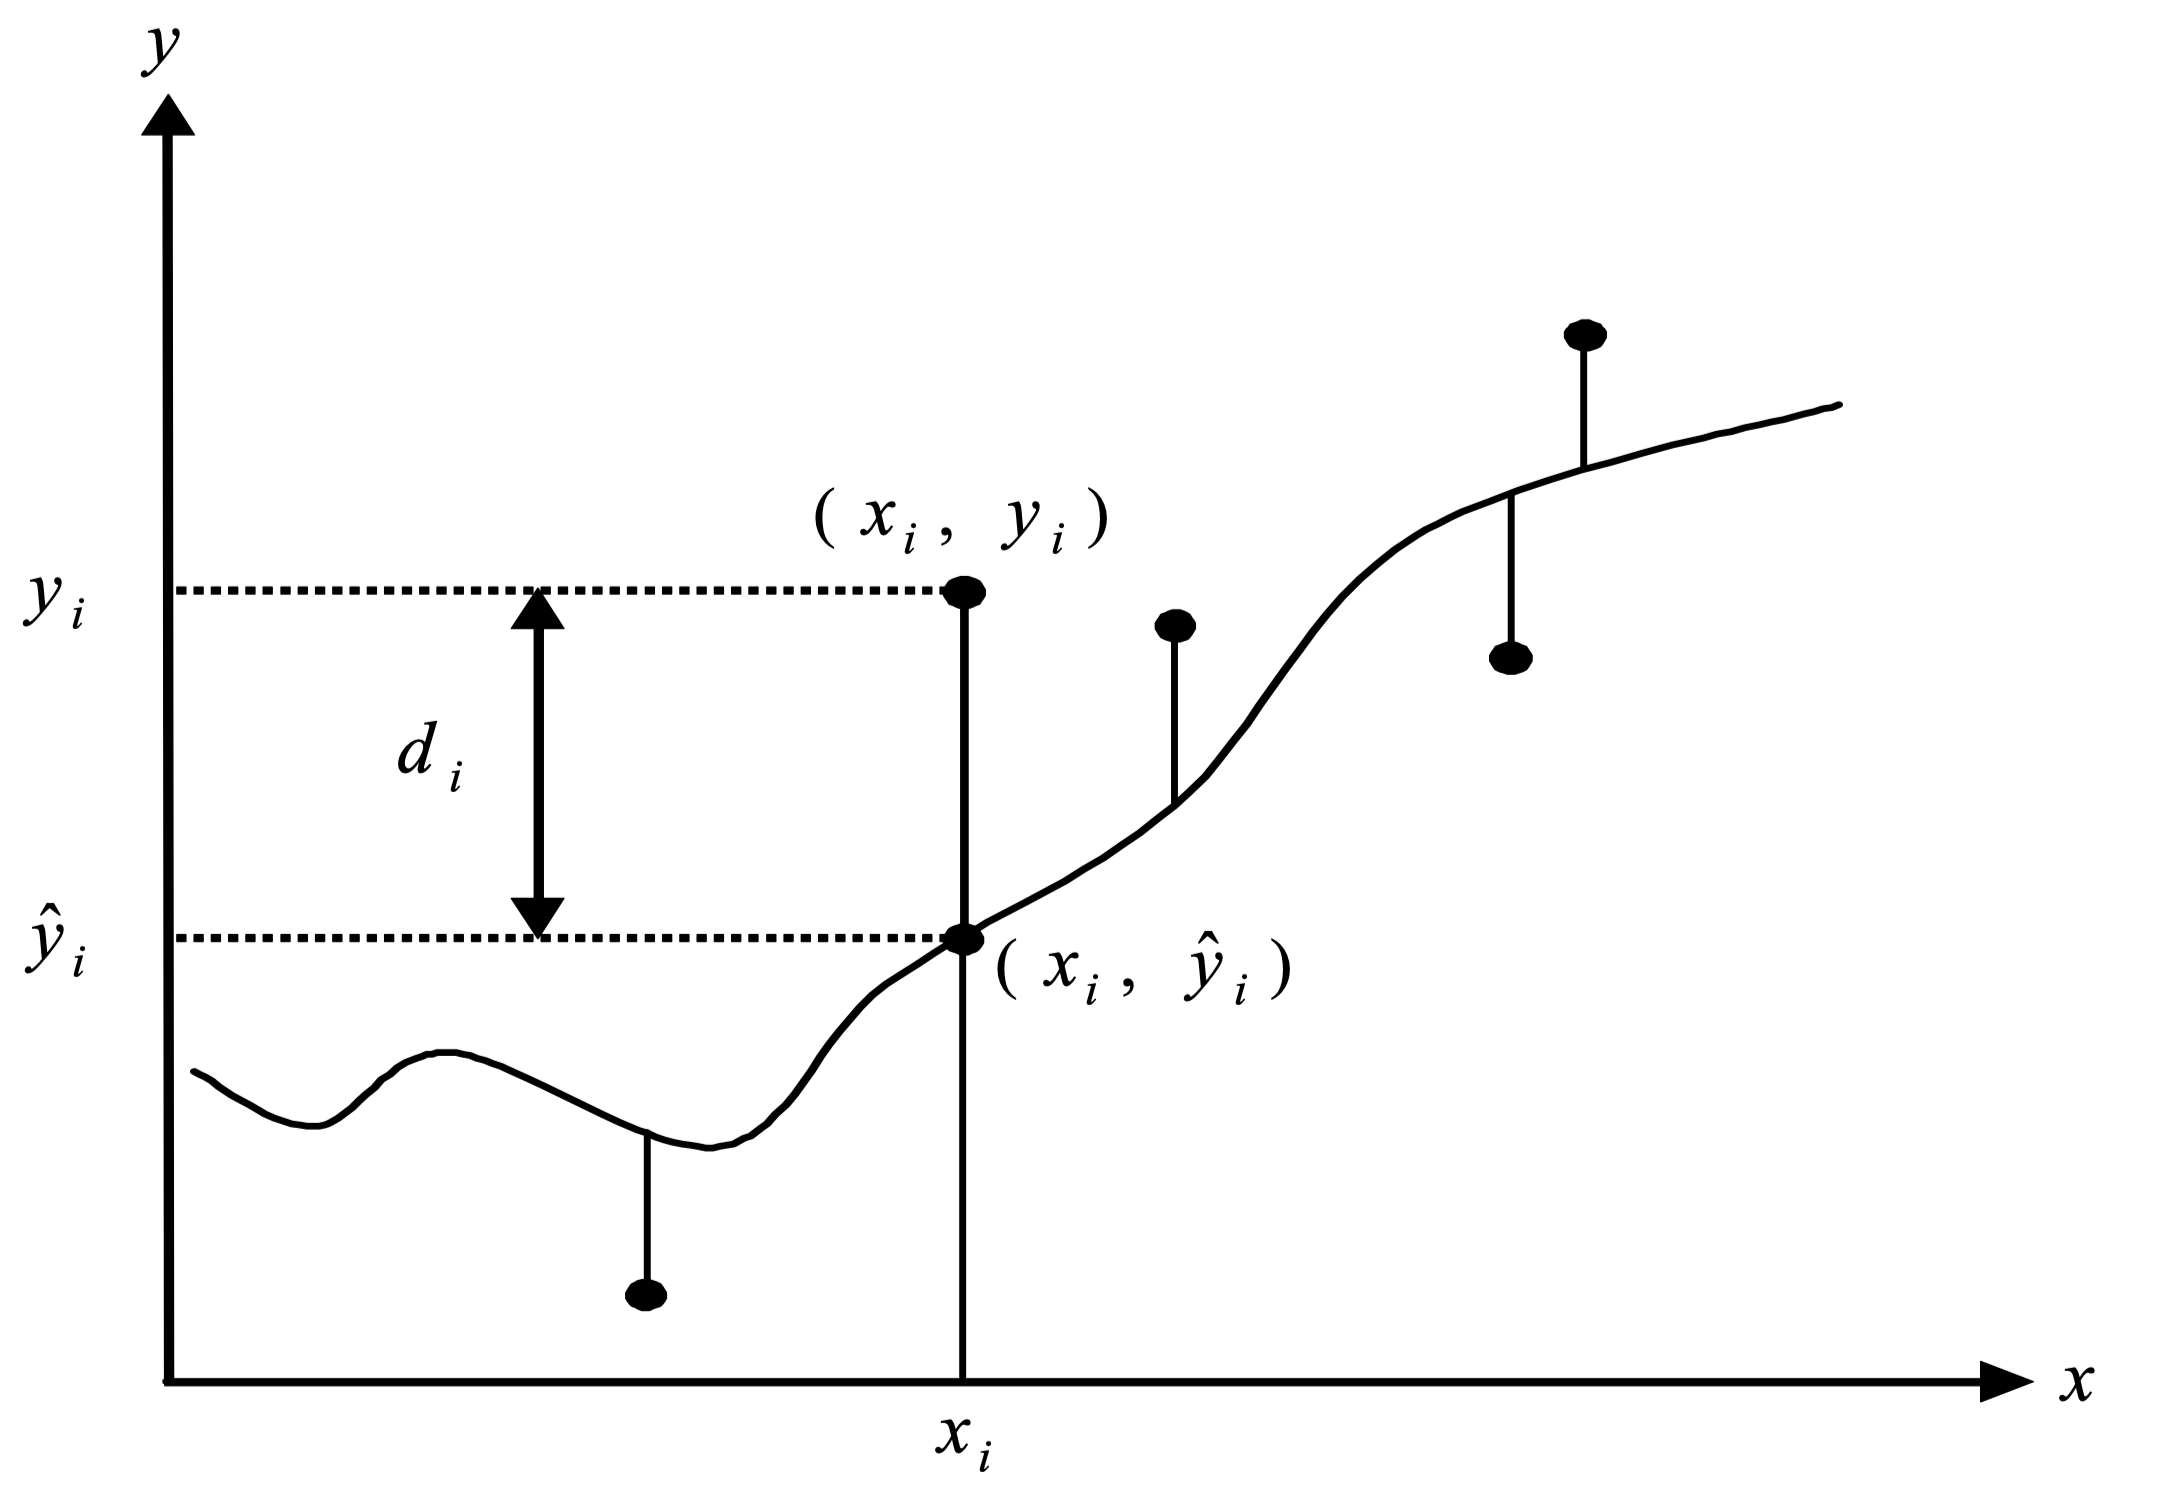
\includegraphics[width=0.75\textwidth,height=\textheight,keepaspectratio]{img/minimi_quadrati.png}
\caption{Condizione dei \textit{minimi quadrati} \cite{excel_per_statistica_belluco}}
\label{fig:minimi_quadrati}
\end{figure}

%La regressione è una tecnica statistica che serve a stimare la relazione esistente tra due o più variabili. In particolare, la regressione permette di individuare il coefficiente di correlazione tra due variabili e di determinare se questa relazione è casuale o no.
%
%Tra le applicazioni principali della regressione ci sono:
%
%- Stima della relazione tra due variabili
%
%- Analisi della relazione tra variabili
%
%- Valutazione dell'influenza di una variabile sulle altre
%
%- Predicting

\subsection{Regressione lineare}\label{ssec:regressione-lineare}
Per stimare la relazione tra due variabili, la regressione lineare utilizza una formula matematica che calcola la media dei valori della prima variabile (Y) in funzione dei valori della seconda variabile (X). La formula della regressione lineare è:

Y = a + bX

In questa formula, a è la costante di regressione e b è la coefficiente di regressione. La costante di regressione a indica la media dei valori di Y in funzione dei valori di X. Il coefficiente di regressione b indica la relazione tra le due variabili: più è vicino a 1, più le due variabili sono correlate in modo lineare.

Utilizzando la regressione lineare, è possibile stimare la relazione tra due variabili anche in presenza di deviazioni dalla linea.

\subsection{Regressione lineare robusta (Huber)}\label{ssec:regressione-huber}
La regressione Huber (in inglese Huber regression, anche detta regressione robusta) è una metodologia statistica per la stima dei parametri di un modello lineare, in presenza di outliers.

Il metodo Huber si basa sul principio della massima verosimiglianza, e si propone di ridurre la sensibilità dei parametri alla presenza di outliers. In particolare, la regressione Huber utilizza una funzione di peso, detta funzione di Huber, che tiene conto della variabilità dei dati intorno ai valori centrali.

\subsection{Regressione lineare avanzata (con rimozione di outlier)}\label{ssec:regressione-cook}
La regressione con rimozione outlier tramite distanza di Cook è una tecnica statistica per ridurre l'influenza degli outliers nei dati di una regressione lineare.

Si basa sul concetto di distanza di Cook, che misura la distanza tra un dato e il valore medio dei dati della stessa variabile. In presenza di outliers, la distanza di Cook aumenta, e quindi questi dati hanno un maggiore impatto sulle stime dei parametri della regressione.

La regressione con rimozione outlier tramite distanza di Cook si basa sull'utilizzo di una funzione di peso, detta funzione di Cook, che tiene conto della distanza di Cook dei dati. La funzione di peso viene utilizzata per ridurre l'influenza degli outliers nei dati della regressione.

\subsection{Regressione Lasso}\label{ssec:regressione-lasso}
La regressione Lasso (in inglese Lasso regression) è una metodologia statistica per la stima dei parametri di un modello lineare, in presenza di outliers.

Il metodo Lasso si basa sul principio della massima verosimiglianza, e si propone di ridurre la sensibilità dei parametri alla presenza di outliers. In particolare, la regressione Lasso utilizza una funzione di peso, detta funzione di Lasso, che tiene conto della variabilità dei dati intorno ai valori centrali.

\subsection{Regressione Ridge}\label{ssec:regressione-ridge}
\ldots

\subsection{Regressione polinomiale}\label{ssec:regressione-polinomiale}
La regressione polinomiale è una generalizzazione della regressione lineare, in cui il rapporto tra Y e X non è più una linea retta.

% Esperimenti e risultati ottenuti
\section{Esperimenti e risultati ottenuti}\label{sec:esperimenti}
\ldots

\subsection{NO2}\label{ssec:risultati-no2}
\ldots

\subsection{PM2.5}\label{ssec:risultati-pm2.5}
\ldots

\subsection{PM10}\label{ssec:risultati-pm10}
\ldots

% Validazione
\section{Validazione}\label{sec:validazione}
\ldots

\subsection{PM2.5}\label{ssec:validazione-pm2.5}
\ldots

\subsection{PM10}\label{ssec:validazione-pm10}
\ldots

% Discussione
\section{Discussione}\label{sec:discussione}
\ldots